%\documentclass{book}
%\usepackage{pgfplots}
%\usepackage[justification=centering]{caption}
%\pgfplotsset{compat=newest}
%\begin{document}
For our experimental evaluation we used both real life database and synthetic database from database repository [\ref{bib:dataset}]. Table [\ref{table:dataset}] shows the data base type and properties.
\begin{table}[t]
\centering
\begin{tabular}{|l|l|l|l|l|}
\hline 
\textbf{Name}&\textbf{Type}&\textbf{Density}&\textbf{Total Transaction} &\textbf{Distinct Items}\\ \hline
mushroom	&	real	&	dense	&	8124	&	120\\ \hline
kosarak	&	real	&	sparse	&	990002	&	41270\\ \hline
pumsb star	&	real	&	sparse	&	49046	&	2088\\ \hline
chess	&	real	&	dense	&	3196	&	75\\ \hline
T10I4D100K	&	synthetic	&	sparse	&	100000	&	869\\ \hline
	\end{tabular}
\caption{Dataset from repository [\ref{bib:dataset}]}
\label{table:dataset}
\end{table}
\subsection{Real Life Data Set}
For real life data sets we have used mushroom [\ref{bib:dataset}], chess [\ref{bib:dataset}] and pumsb star [\ref{bib:dataset}]. Mushroom, chess and pumsb star are dense datasets. Mushroom has 8124 transactions with 120 distinct items, chess has 3196 transactions with 75 distinct items and pumsb star has 49046 transactions with 2088 distinct items. For probability assignment to each items we used normal distribution for getting existential probability.
\subsection{Synthetic Data Set}
For synthetic data sets we have used T10I4D100K [\ref{bib:dataset}]. It is an IBM generated transactional data set widely used for frequent pattern mining. It is a sparse data set with 100000 transactions and 869 distinct items. For probability assignment to each items we used normal distribution for getting existential probability.
%%mark = star, diamond, square, otimes
%\documentclass{article}
%\usepackage{pgfplots}
%\usepackage[justification=centering]{caption}
%\pgfplotsset{compat=newest}
%\begin{document}
\begin{figure}
\centering

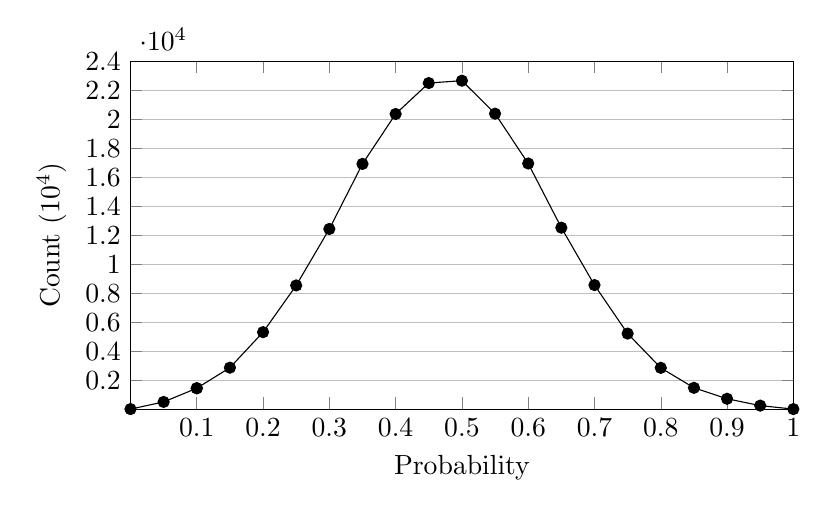
\begin{tikzpicture}
\begin{axis}[
 width=10cm,
   height=6cm,
    xlabel={Probability },
    ylabel={Count ($10^4$)},
    xmin=0, xmax=1.0,
    ymin=0, ymax=24000,
    xtick={.1,.2,.3,.4,.5,.6,.7,.8,.9,1.0},
    ytick={2000,4000,6000,8000,10000,12000,14000,16000,18000,20000,22000,24000},
    legend pos=north east,
    ymajorgrids=true,
    grid style={line width=.2pt,draw=gray!50},
]
 
\addplot[
    solid, every mark/.append style={solid, fill=black}, mark=*
    ]
    coordinates {
		(0,0)
		(.05,495)
		(0.1,1439)
		(0.1 ,1439)
		(0.15,2859)
		(0.2 ,5307)
		(0.25,8531)
		(0.3 ,12426)
		(0.35,16915)
		(0.4 ,20358)
		(0.45,22493)
		(0.5 ,22655)
		(0.55,20380)
		(0.6 ,16943)
		(0.65,12514)
		(0.7 ,8555)
		(0.75,5209)
		(0.8 ,2845)
		(0.85,1468)
		(0.9 ,712)
		(0.95,240)
		(1.0,0)
};
 
\end{axis}
\end{tikzpicture}
%\caption{Probability Distribution for \emph{Mushroom} data set}
\label{result:data_mushroom}
\end{figure}
%\end{document}
%%mark = star, diamond, square, otimes
%\documentclass{article}
%\usepackage{pgfplots}
%\usepackage[justification=centering]{caption}
%\pgfplotsset{compat=newest}
%\begin{document}
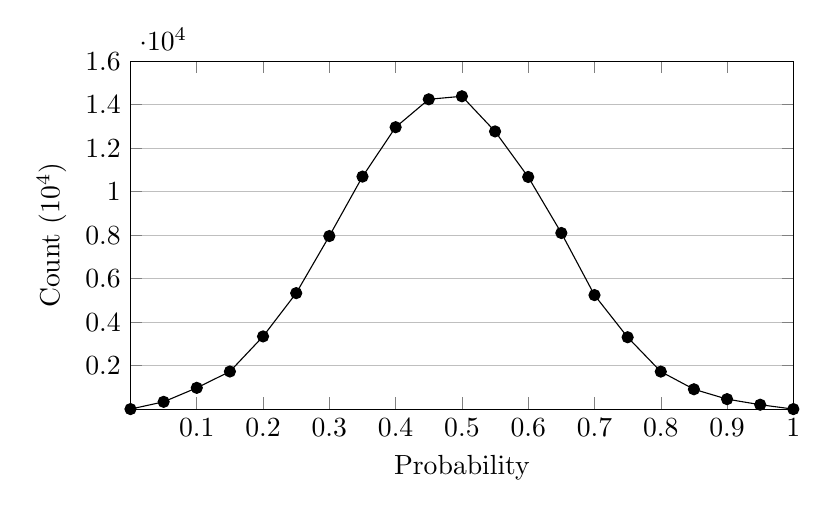
\begin{tikzpicture}
\begin{axis}[
 width=10cm,
   height=6cm,
    xlabel={Probability },
    ylabel={Count ($10^4$)},
    xmin=0, xmax=1.0,
    ymin=0, ymax=16000,
    xtick={.1,.2,.3,.4,.5,.6,.7,.8,.9,1.0},
    ytick={2000,4000,6000,8000,10000,12000,14000,16000},
    legend pos=north east,
    ymajorgrids=true,
    grid style={line width=.2pt,draw=gray!50},
]
 
\addplot[
    solid, every mark/.append style={solid, fill=black}, mark=*
    ]
    coordinates {
			(0,0)
			(0.05,334)
			(0.1,977)
			(0.15,1729)
			(0.2,3342)
			(0.25,5333)
			(0.3,7958)
			(0.35,10692)
			(0.4,12964)
			(0.45,14247)
			(0.5,14386)
			(0.55,12770)
			(0.6,10675)
			(0.65,8099)
			(0.7,5242)
			(0.75,3304)
			(0.8,1724)
			(0.85,912)
			(0.9,458)
			(0.95,201)
			(1,0)

};
 
\end{axis}
\end{tikzpicture}
%\end{document}
%%mark = star, diamond, square, otimes
%\documentclass{article}
%\usepackage{pgfplots}
%\usepackage[justification=centering]{caption}
%\pgfplotsset{compat=newest}
%\begin{document}
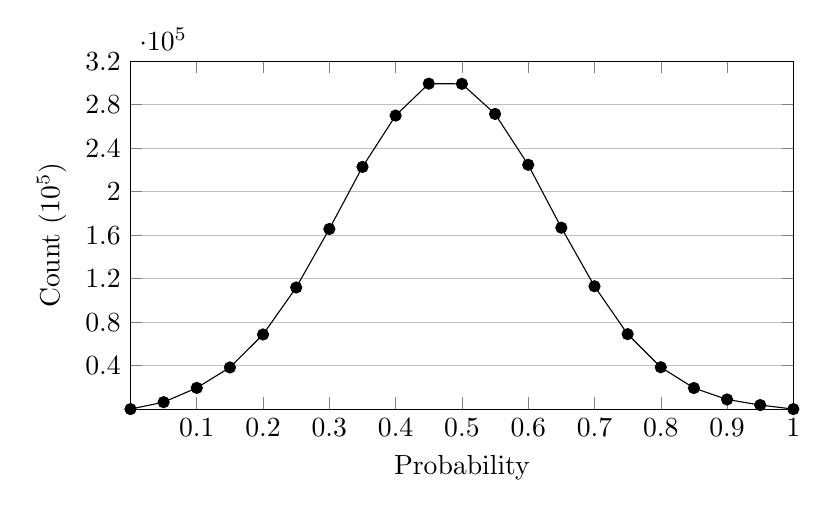
\begin{tikzpicture}
\begin{axis}[
 width=10cm,
   height=6cm,
    xlabel={Probability },
    ylabel={Count ($10^5$)},
    xmin=0, xmax=1.0,
    ymin=0, ymax=320000,
    xtick={.1,.2,.3,.4,.5,.6,.7,.8,.9,1.0},
    ytick={40000,80000,120000,160000,200000,240000,280000,320000},
    legend pos=north east,
    ymajorgrids=true,
    grid style={line width=.2pt,draw=gray!50},
]
 
\addplot[
    solid, every mark/.append style={solid, fill=black}, mark=*
    ]
    coordinates {
			(0,0)
			(0.05,6362)
			(0.1,19508)
			(0.15,38310)
			(0.2,68623)
			(0.25,111854)
			(0.3,165662)
			(0.35,222758)
			(0.4,269985)
			(0.45,299328)
			(0.5,299159)
			(0.55,271454)
			(0.6,224689)
			(0.65,166840)
			(0.7,112959)
			(0.75,68933)
			(0.8,38490)
			(0.85,19368)
			(0.9,8848)
			(0.95,3707)
			(1,0)
};
 
\end{axis}
\end{tikzpicture}
%\end{document}
%mark = star, diamond, square, otimes
%\documentclass{article}
%\usepackage{pgfplots}
%\usepackage[justification=centering]{caption}
%\pgfplotsset{compat=newest}
%\begin{document}
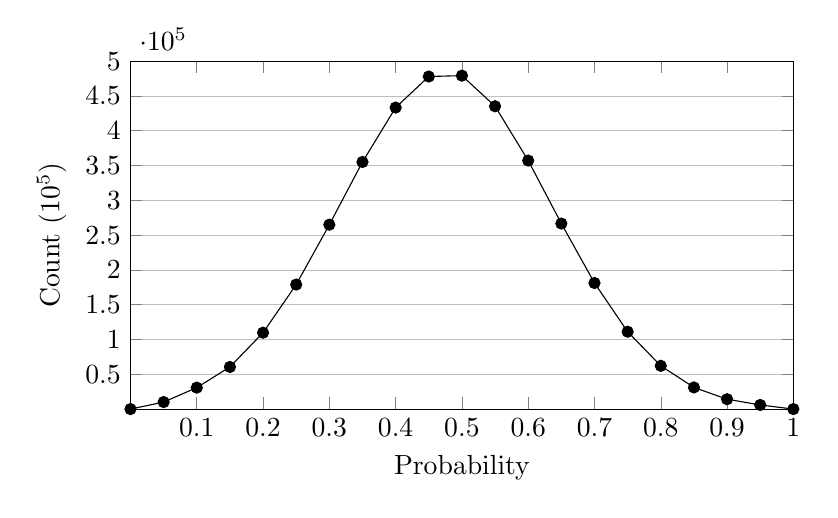
\begin{tikzpicture}
\begin{axis}[
 width=10cm,
   height=6cm,
    xlabel={Probability },
    ylabel={Count ($10^5$)},
    xmin=0, xmax=1.0,
    ymin=0, ymax=500000,
    xtick={.1,.2,.3,.4,.5,.6,.7,.8,.9,1.0},
    ytick={50000,100000,150000,200000,250000,300000,350000,400000,450000,500000},
    legend pos=north east,
    ymajorgrids=true,
    grid style={line width=.2pt,draw=gray!50},
]
 
\addplot[
    solid, every mark/.append style={solid, fill=black}, mark=*
    ]
    coordinates {
			(0,0)
			(0.05,10068)
			(0.1,30825)
			(0.15,60529)
			(0.2,109792)
			(0.25,178975)
			(0.3,265006)
			(0.35,355127)
			(0.4,433334)
			(0.45,477961)
			(0.5,479225)
			(0.55,435233)
			(0.6,357179)
			(0.65,266639)
			(0.7,181169)
			(0.75,111182)
			(0.8,62178)
			(0.85,31116)
			(0.9,14207)
			(0.95,5909)
			(1,0)
};
 
\end{axis}
\end{tikzpicture}
%\end{document}
%\end{document}